\documentclass[conference]{IEEEtran}
\IEEEoverridecommandlockouts
% The preceding line is only needed to identify funding in the first footnote. If that is unneeded, please comment it out.
\usepackage{cite}
\usepackage{amsmath,amssymb,amsfonts}
\usepackage{algorithmic}
\usepackage{graphicx}
\usepackage{textcomp}
\usepackage{xcolor}
\usepackage{booktabs}
\usepackage{comment}
\usepackage{url}

\def\BibTeX{{\rm B\kern-.05em{\sc i\kern-.025em b}\kern-.08em
    T\kern-.1667em\lower.7ex\hbox{E}\kern-.125emX}}
\begin{document}

\title{Enhancing Product Recommendations with Multi-Modal LLMs
}

\author{
\IEEEauthorblockN{Babaniyi Olaniyi}
\IEEEauthorblockA{
Department of Statistics and Mathematical Sciences \\
Kwara State University \\
Ilorin, Nigeria
}
}


\maketitle

\begin{abstract}

Recommender systems increasingly benefit from multimodal signals such as text and images, which provide richer context about users and items than interactions alone. In this work, we present \textit{MM-GPT2Rec}, a multimodal sequential recommender built from scratch by fine-tuning GPT-2 (``gpt2-medium'') to predict users' next likely purchases. Each product is represented through a joint text–image embedding, and sequences of user interactions are modeled analogously to word sequences in language. We conduct comprehensive evaluation using multiple runs, statistical significance testing, and confidence intervals to ensure credible results. Evaluated on an Amazon product dataset (100K+ interactions), MM-GPT2Rec outperforms comprehensive baselines including traditional methods (collaborative filtering, matrix factorization, hybrid, popularity, content-based) and multimodal baselines (VBPR, DeepCoNN, NRMF, SASRec) on accuracy-focused metrics. Ablation studies demonstrate the contribution of individual modalities and fusion methods. Beyond accuracy, our model achieves substantially higher catalog coverage and diversity than CF-based methods, though with slightly lower novelty compared to pure content-based recommendations, highlighting a trade-off between relevance and exploration. These results demonstrate the effectiveness of leveraging multimodal signals within a transformer architecture for recommendation, and suggest that scaling to larger foundation models and end-to-end multimodal encoders could further advance the state of sequential recommendation. 

\end{abstract}



\begin{IEEEkeywords}
Recommender systems, Multimodal learning, Sequential recommendation, Transformer models, Large language models, Deep learning, Collaborative filtering, Personalization, Information retrieval, Natural language processing
\end{IEEEkeywords}

%The implementation of MM-GPT2Rec is publicly available.\footnote{\url{https://github.com/babaniyi/multimodal_llm_recsys_amazon}}

\section{Introduction}
Recommender systems (RecSys) play a pivotal role in e-commerce and content platforms by predicting which items a user is likely to interact with next. Traditional recommendation algorithms often rely on patterns in user–item interaction data (e.g. collaborative filtering) or on item attributes (content-based filtering). However, modern platforms offer abundant \textit{multimodal} data such as product images, textual descriptions, and user reviews that can enrich a model’s understanding of user preferences. Incorporating multiple modalities has been shown to improve the relevance of recommendations in practice. For example, eBay reported that by integrating information from item titles (text) and images, they significantly improved the relevance of recommended listings and increased user engagement \cite{b4}. Likewise, academic studies have found that using text reviews or visual features of products can enhance the accuracy of recommendations compared to using only structured ratings or IDs \cite{b5}. Multimodal approaches can alleviate data sparsity and cold-start issues by providing additional signals about items; \textit{e.g.}, images convey visual style or design preferences that ratings alone cannot \cite{b5}.


At the same time, the recommender systems community is exploring the use of large language models (LLMs) and other foundation models as a new paradigm for recommendations.  Large pre-trained models from NLP and CV (e.g. GPT series, BERT, CLIP) capture high-level representations that could be repurposed for user–item modeling \cite{b6}. Transformers in particular have proven effective for sequential recommendations: models such as SASRec and BERT4Rec apply transformer architectures to predict the next item in a user's behaviour sequence, yielding state-of-the-art results on benchmark data sets \cite{b7}. Recent work has even fine-tuned generative language models (such as GPT-2 or GPT-3) for recommendation tasks. For instance, one approach (RecPPT) uses a pretrained GPT-2 to model user histories, introducing new item embeddings and output layers to adapt the language model for recommender data \cite{b8}. Another line of research has proposed "RecGPT" variants that tailor LLMs to recommender systems by fine-tuning interaction data or using prompting strategies \cite{b9}.  These developments suggest that LLMs can serve as powerful sequence models in RecSys, leveraging their capacity to capture complex patterns. 


Motivated by these trends, we explore a \textbf{multimodal LLM-based recommender} under resource-constrained conditions. In this paper, we present a product recommendation system  that integrates textual and visual item information into a GPT-2 medium model to predict the next likely purchase for each user. The key idea is to treat the next-item recommendation problem analogously to next-word prediction in language modeling: each product (item) is represented as a 'token' embedding that encapsulates its text and image characteristics, and a transformer decoder is trained to generate the sequence of items with which a user would interact. The transformer thus learns to continue the user’s purchase sequence, conditioned on their history, by outputting a probability distribution over the next item token. We built this system from scratch and fine-tuned it on a subset of Amazon product data, including review text and product images.

%% TO DO: Update this section with correct values and conclusion after running the model with full data

Our implementation uses GPT-2 (with $\sim$345M parameters) due to GPU memory limitations, but this serves as a proof-of-concept for larger LLMs in recommender settings. We combine user history sequences with multi-modal item embeddings derived from pre-trained text and vision models. The resulting model (which we refer to as \textit{MM-GPT2Rec}) \footnote{Implementation available at: \url{https://github.com/babaniyi/multimodal_llm_recsys_amazon}} is evaluated against a variety of baseline recommenders: user and item-based collaborative filtering, content-based filtering using the same item metadata, a hybrid approach, a popularity-based model, and a matrix factorization method. We report evaluation on Top-$N$ recommendation metrics (Hit Rate@10, Precision@10, Recall@10, NDCG@10, MRR, MAP) as well as \textit{beyond-accuracy} measures (Coverage, Diversity, Novelty) to provide a comprehensive comparison.


Our experiments, though limited in scale, show that the proposed multimodal \textit{MM-GPT2Rec} consistently outperforms all baseline models on accuracy-oriented metrics at $k=10$. In particular, it achieves perfect hit rate (HR@10 = 1.0), the highest NDCG@10 (3.93), and strong precision (0.813), demonstrating its ability to accurately predict users’ next purchases. These gains stem from the model’s rich multimodal representations: for example, it can infer that a user who purchased a phone case and screen protector is likely to buy another complementary accessory with a matching design, by combining image features and textual review signals. We find that incorporating both reviews and images enables substantially more precise modeling of user preferences than relying on either modality alone. At the same time, our analysis highlights important trade-offs. A pure content-based recommender, while weaker in accuracy, yields higher diversity by surfacing a wider range of items across users’ recommendation lists. In contrast, \textit{MM-GPT2Rec} tends to prioritize relevance often recommending popular or closely related items which boosts ranking quality but reduces intra-list variety. Understanding this trade-off between accuracy and diversity \cite{b10} is essential for guiding the practical deployment of LLM-based recommenders.



The contributions of this paper are summarized as follows:
\begin{itemize}
    \item We develop a novel multi-modal sequential recommendation model using a GPT-2 transformer, demonstrating how a pre-trained language model architecture can be adapted for next-item prediction by encoding items as sequences of text and image features.

    \item  We design a data processing pipeline that combines Amazon product reviews (textual modality) and product images (visual modality) to create unified item embeddings. These are used to train the \textit{MM-GPT2Rec} model on a real-world dataset of user purchase histories.

    \item We provide an extensive evaluation across standard top-$N$ metrics and beyond-accuracy metrics, benchmarking the proposed approach against multiple baseline algorithms (collaborative filtering, content-based, hybrid, popularity, matrix factorization). This offers insights into where a multimodal LLM-based recommender excels and where it needs improvement.

    \item We highlight the limitations of using a mid-sized model like GPT-2 on limited data, and suggest future improvements, including scaling to larger LLMs (GPT-3, GPT-4, etc.), using multimodal transformers that natively handle image inputs, and incorporating techniques to improve recommendation novelty and diversity.

    
\end{itemize}


The remainder of the paper is organized as follows. In Section 2, we review related work on large language models in recommender systems and prior approaches to multimodal recommendation. Section 3 describes our methodology, including the dataset, feature extraction process, and the architecture of the \textit{MM-GPT2Rec} (with an overview diagram of the system). Section 4 presents the experimental setup and results, comparing our model to baselines. Section 5 provides a discussion of the results and analyzes the model’s performance on various metrics, with an emphasis on where the multi-modal LLM approach provides benefits and where it has trade-offs. Section 6 outlines the limitations of our current implementation and proposes directions for future work, and finally Section 7 concludes the paper.




\section{Related Work}
\subsection{Large Language Models in Recommendation Systems}
The surge of large-scale pre-trained models in NLP has sparked interest in applying these models to recommendation problems. Large Language Models (LLMs) like GPT-2, GPT-3, BERT, etc., are capable of capturing complex patterns from sequences, which naturally aligns with tasks such as sequential recommendation or session-based recommendation. Several researchers have explored using LLMs to improve recommender systems. One approach is to use LLMs without additional training (zero-shot or few-shot) by carefully prompting them with a user’s history or profile and asking for recommendations; while intriguing, this approach often struggles as LLMs are not explicitly trained on the target item space. A more direct approach is fine-tuning or adapting LLMs on recommender data. \cite{b7} introduced \textbf{BERT4Rec}, a bidirectional transformer model for sequential recommendation, which uses the BERT architecture and a Cloze (masking) training objective to predict items within sequences. BERT4Rec demonstrated that transformer-based models can outperform earlier sequential models (such as RNN or CNN-based recommenders), effectively learning user behavior patterns.

Building on this idea, recent works have attempted to leverage \textit{causal} language models (unidirectional generative models). For example, \textbf{SASRec} (Self-Attention Sequential Rec) uses a unidirectional transformer similar to the decoder part of GPT to predict the next item in a sequence, showing the benefit of the “Attention is All You Need” architecture for recency-aware recommendations \cite{b7}. More recent is \textbf{RecPPT}, which explicitly uses GPT-2’s architecture and partially its pre-trained weights for sequential recommendation. RecPPT “reprograms” a GPT-2 model by replacing its input embedding matrix and output vocabulary with item embeddings, while leveraging the pretrained transformer layers to model the sequence \cite{b8}. This method essentially treats item IDs as a new language to be learned by the GPT model, a strategy that our approach also adopts. Meanwhile, \textbf{RecGPT} focuses on using instruction-tuning and chat-based frameworks (e.g., adapting ChatGPT or LLaMA) to engage in conversational recommendation or to generate personalized prompts \cite{b9}. These works point toward a future where recommender systems have their own foundation models or leverage general foundation models for improved reasoning and understanding of context.

However, fully fine-tuning giant LLMs (with billions of parameters) on recommendation datasets can be prohibitive; research is ongoing into efficient tuning (e.g. via LoRA or prompt tuning) and into \textit{domain-adaptive pre-training} for recommendation. Our work specifically fine-tunes a medium-sized GPT-2 (345M params) due to computational limits, but it demonstrates the feasibility of this approach. We contribute to this line by incorporating multi-modal inputs, whereas most prior LLM-for-RecSys studies focus on textual or ID-only data. A parallel development worth noting is the idea of using LLMs to generate synthetic data or augment sparse training data for cold-start scenarios, which we do not explore here but could complement our method.


\subsection{Multi-modal Recommendation Systems}
Integrating multiple data modalities into recommender systems has been a topic of interest for over a decade. Early work in this area dealt with improving recommendations by using content features such as text from item descriptions or images for visual appeal. For example, \textbf{VBPR} (Visual Bayesian Personalized Ranking) \cite{b12} extracted visual features from product images and incorporated them into a matrix factorization model, which improved recommendations especially for fashion items and helped with cold start for new items \cite{b5}. The intuition is that users often have consistent preferences in the visual domain (clothing style, color, etc.), so leveraging image embeddings can capture those aspects. Similarly, text reviews and product descriptions have been used to enhance recommenders: \textbf{DeepCoNN} (Deep Cooperative Neural Networks) and \textbf{NRMF} (Neural Rating \& Meta-data Fusion) are examples of models that use review text to learn better user and item representations, which in turn improve rating prediction or Top-$N$ recommendation. Studies have shown that models incorporating review text significantly outperform those using only ratings, confirming that reviews provide rich preference signals.

More recent research has looked at combining multiple modalities simultaneously. For instance, \textbf{CAMRec} (Contextual Attention Multi-modal Rec) by \cite{b5} uses both textual and visual features of products: it employs RoBERTa to encode review text and VGG-16 to encode product images, then applies a co-attention mechanism to fuse these features \cite{b5}. The fused item representation is used alongside user interaction history to predict ratings. Their findings indicate that using both modalities yields a more accurate reflection of user preferences than single-modality models. In their experiments on Amazon Electronics data, the multi-modal model provided better rating predictions than text-only or image-only baselines, and even improved upon strong baselines like Neural CF or review-based models.

Beyond academic examples, industry systems (as mentioned for eBay) have also deployed multi-modal embeddings to great effect \cite{b4}. A common approach in industry is the two-tower model, where one tower processes text (e.g. product title embeddings via BERT) and another processes images (via ResNet), and they are combined to produce a unified item embedding. This embedding can then be used in various stages of the recommendation pipeline, from candidate retrieval to ranking. The multimodal two-tower architecture has been reported to improve relevance by ensuring that both the visual and textual aspects of an item match the query or the user's interest.

Our work contributes to multimodal recommendation research by demonstrating a unified architecture where multi-modal item features are directly fed into a sequential recommender model. One closely related contemporary work is by \cite{b15}), who propose a \textit{multi-modal clothing recommendation model} that also utilizes a pre-trained large language model for analyzing text+image inputs \cite{b15}. They integrate clothing description texts and images, using a large language model to “deeply explore the hidden meanings” of user and product information, and additionally use a variational autoencoder to model user–product relationships for cold start. Their results showed significant performance gains over traditional methods, highlighting the promise of combining LLMs with multi-modal data in RecSys. We share a similar spirit but focus on the sequential recommendation task (next-item prediction) and use GPT-2 as the sequence model core. Finally, we note that our evaluation includes metrics for diversity and novelty, which connect to a broad literature on beyond-accuracy objectives in recommender systems \cite{b11}. Multi-modality can influence these metrics in complex ways: on one hand, having more item features could help a model recommend a wider range of items (potentially increasing catalog coverage and diversity); on the other hand, if not carefully regularized, a powerful model might over-concentrate on popular patterns (potentially decreasing novelty of recommendations). We use standard definitions of these metrics: diversity is typically defined as the dissimilarity among items recommended to the same user \cite{b10}, and novelty measures how unexpected or long-tail the recommended items are for the user. Balancing accuracy with diversity and novelty remains an important challenge, and we discuss how our multi-modal GPT-2 model fares in this regard compared to a content-based approach. 



\subsection{Baseline Recommendation Techniques}
To put our contributions in context, we briefly recap the baseline techniques against which we compare:
\begin{itemize}
\item \textbf{Popularity-based}: A non-personalized method that recommends the globally most popular items (highest overall purchase counts). This often serves as a simple baseline; it tends to have very low coverage (since only a handful of items are recommended to everyone) \cite{b10} and low novelty (recommending mostly best-sellers), but it can achieve surprisingly decent hit rates in some datasets where many users gravitate to popular items.

\item \textbf{Collaborative Filtering (User-based \& Item-based)}: User-based CF finds neighbors of the target user (based on similarity in past item interactions) and recommends items that those neighbors liked. Item-based CF finds items similar to those the user has consumed and recommends similar items. We implement these using cosine similarity on the user-item interaction matrix. CF can personalize recommendations but may struggle with new items or new users (cold start) and often does not incorporate content.

\item \textbf{Content-based Filtering}: This method recommends items that are similar in content to what the user has liked in the past. In our setting, we utilize the textual and visual features of items to define similarity. Essentially, we compute a profile for each user by aggregating the features of items they have purchased, and recommend new items whose feature vectors are closest to the user’s profile vector (e.g., by cosine similarity). Content-based methods naturally excel at recommending niche items that fit a user’s specific interests (thus often improving novelty), but they might miss broader trends or popular items that the user might also like but are outside their profile. They also require rich content features to be effective.

\item \textbf{Hybrid Recommender}: A combination of collaborative and content-based signals. Many hybrid designs exist; in our experiment, we implement a simple hybrid by averaging the normalized scores from an item-based CF and the content-based recommender for each candidate item, then recommending top items by this combined score. The intuition is to leverage both the wisdom of the crowd (CF) and the specific content preferences of the user.

\item \textbf{Matrix Factorization (MF)}: A classic model-based CF approach where users and items are represented as latent vectors, learned by factorizing the interaction matrix. We specifically use a variant of \textit{implicit} MF optimized for top-$N$ recommendation (like BPR ~\cite{b13} or ALS on implicit feedback). MF captures user taste and item characteristics in latent dimensions and can generalize better than memory-based CF on sparse data. However, standard MF does not use any content features, so it purely relies on interaction patterns.

\item \textbf{Neural Network Baselines}: We also mention that advanced baselines like \textbf{NeuMF} (Neural Matrix Factorization) combine MF with a multi-layer perceptron for CF~\cite{b12}, and \textbf{Deep Hybrid} models exist which combine content and CF via neural architectures. Due to resource limits, we did not implement complex neural baselines beyond our proposed model; our focus is on comparing to interpretable and representative traditional methods. From prior work, we note that neural CF models can outperform basic MF if enough data is available \cite{b5}, and they can be extended with content inputs as in \textbf{DeepCoNN} or \textbf{DSSM}-style recommenders.
\end{itemize}


In summary, the literature suggests that (1) multi-modal features help recommendations by providing richer signals about items and users’ preferences, and (2) LLMs and transformers offer a powerful way to model sequential behavior and possibly understand content. Our work stands at this intersection, evaluating whether a transformer-based LLM (GPT-2) can effectively merge multi-modal content into a coherent next-item prediction model, and how it compares with traditional approaches.



\section{Methodology}

In this section, we describe the proposed multi-modal recommendation system, including the data preprocessing pipeline, the construction of multi-modal item embeddings, the architecture of the GPT-2 based sequence model, and the training procedure. We also illustrate the overall system design and data flow. Figure~\ref{fig:architecture} provides a high-level overview of the system architecture, showing how user histories and item features are processed to produce next-item recommendations.



\subsection{Dataset and Preprocessing}
We evaluated our approach on a subset of the Amazon Product dataset \cite{b14}, a public collection of Amazon product reviews and metadata. Specifically, we selected a single category ("Appliances") for manageability, though our methodology is general and can be applied to other categories. Our dataset contains 100,000+ user-item interactions, representing a significant scale improvement from typical small-scale evaluations. The raw data for this category includes (i) user review records (user ID, item ID, rating, timestamp, review text, etc.), (ii) product metadata (item title, category taxonomy, price, brand), and (iii) product images (each item has one or more product images available). For our purposes, the key fields were user IDs, item IDs, timestamps, review text, and product images. We ignored ratings in training (treating all interactions as implicit feedback), and we did not use category labels or prices in the current model, focusing only on free-form text and image content to represent items.

Our framework supports datasets up to 500K interactions, demonstrating scalability beyond the original 40K limit. We use a temporal split of 75\% train, 15\% validation, and 10\% test, with a minimum of 7 interactions per user to ensure meaningful user profiles.

%\subsection{Data Processing - Processing Layer}
%Our framework consists of two main components, the text encoder and the image encoder, which work together to provide product recommendations.

%\subsection{Models Used - Baselines}
%
%\subsection{Problem Formulation}
%Consider a system of $I$ users and $J$ items. We use a vector $p_{j}$ to denote the list of sequential items $J$ purchased by the user $i$. %Furthermore, we use $x_{i}^{u}x_{j}^{v}$ to denote the textual features associated with user $i$ and item $j$, such as the user review $i$' and %the features of item $j$', such as image, brand, price, description, etc. 

%Similar to \cite{b3}, our goal is to design a generative recommender system that tightly couples LLMs with the recommendation %task by introducing user/item ID tokens (and token embeddings), such that the semantics of the user/item (for example, users' interests in an %item) can be accurately modeled for efficient and effective recommendations, and the encoded knowledge and reasoning ability of pre-trained LLMs %can be fully used simultaneously.

%% TODO: Review this section. These are placeholders
\paragraph{Text Processing} Each item in our subset consists of a title and a set of review texts. To enrich our dataset, we filter the data to include only transactions from users with at least three reviews. We then utilize a pretrained language model to generate a semantic embedding of the item's text. Specifically, we employed a \textbf{Byte Pair Encoder} to encode the concatenated text into a fixed-dimensional vector. This choice was made due to its relatively small size and fast inference, which are crucial given our computational constraints. For each user, we retrieve the next ten items they purchased, along with the product images of these items. Additionally, we defined an instruction for the model stating: \textit{"Given a user's purchase history and review for a product, predict the next ten products they are likely to purchase."}


\paragraph{Image Processing} For the visual modality, we obtained one representative product image for each item. (In the Amazon data, each product often has multiple images; we took the main image URL as it has the highest quality) and applied standard transformations: resizing to $224\times256$ and center-cropping to $224\times224$ pixels. To extract visual features, we used a pre-trained \textbf{ResNet-18} CNN.

\paragraph{Multi-modal Item Embeddings} Finally, we combine text and image embeddings into a single vector for each element. We tried two fusion strategies: concatenation vs. element-wise addition. Concatenation ($d_{text} 768$  + $d_{image} 256$ = $1024$) preserves all the information of both modalities and resulted in a embedding of $1024$ dimensional elements. This coincidentally matches the hidden size of GPT-2 medium (which is $1024$), simplifying integration. Element-wise addition, on the other hand, requires the vectors to be of equal size; to test this, we also projected both text and image embeddings to $d=512$ and then added them. We found concatenation followed by a linear layer works slightly better, likely because it allows the model to weight modalities as needed. Therefore, the item’s final embedding $\mathbf{e}_{item}$ is: $e_{item} = W_{f}[e_{text}||e_{image}] + b_{f}$ where $[\cdot||\cdot]$ denotes concatenation, and $W_f$ is a learned $1024\times1024$ matrix (and $b_f$ a bias) that can fuse/transform the concatenated features. We initialize $W_f$ as an identity mapping (and $b_f=0$) so that initially $\mathbf{e}_{item}$ is just the concatenation of text and image features. During training, $W_f$ is fine-tuned, allowing the model to re-weight or mix the modalities optimally (this essentially acts like a simple feed-forward layer on each item embedding).

After this preprocessing, we have:

\begin{enumerate}
    \item A dictionary of item embeddings: for each item ID in our subset, a $d = 1024$ vector representing its multi-modal content.
    \item A set of user sequences (for training): each sequence is a list of item IDs [i$_1$, i$_2$, ..., i$_n$] for that user.
\end{enumerate}

%% TODO: Confirm this
\subsection{Model Architecture}

\begin{figure}[ht]
  \centering
  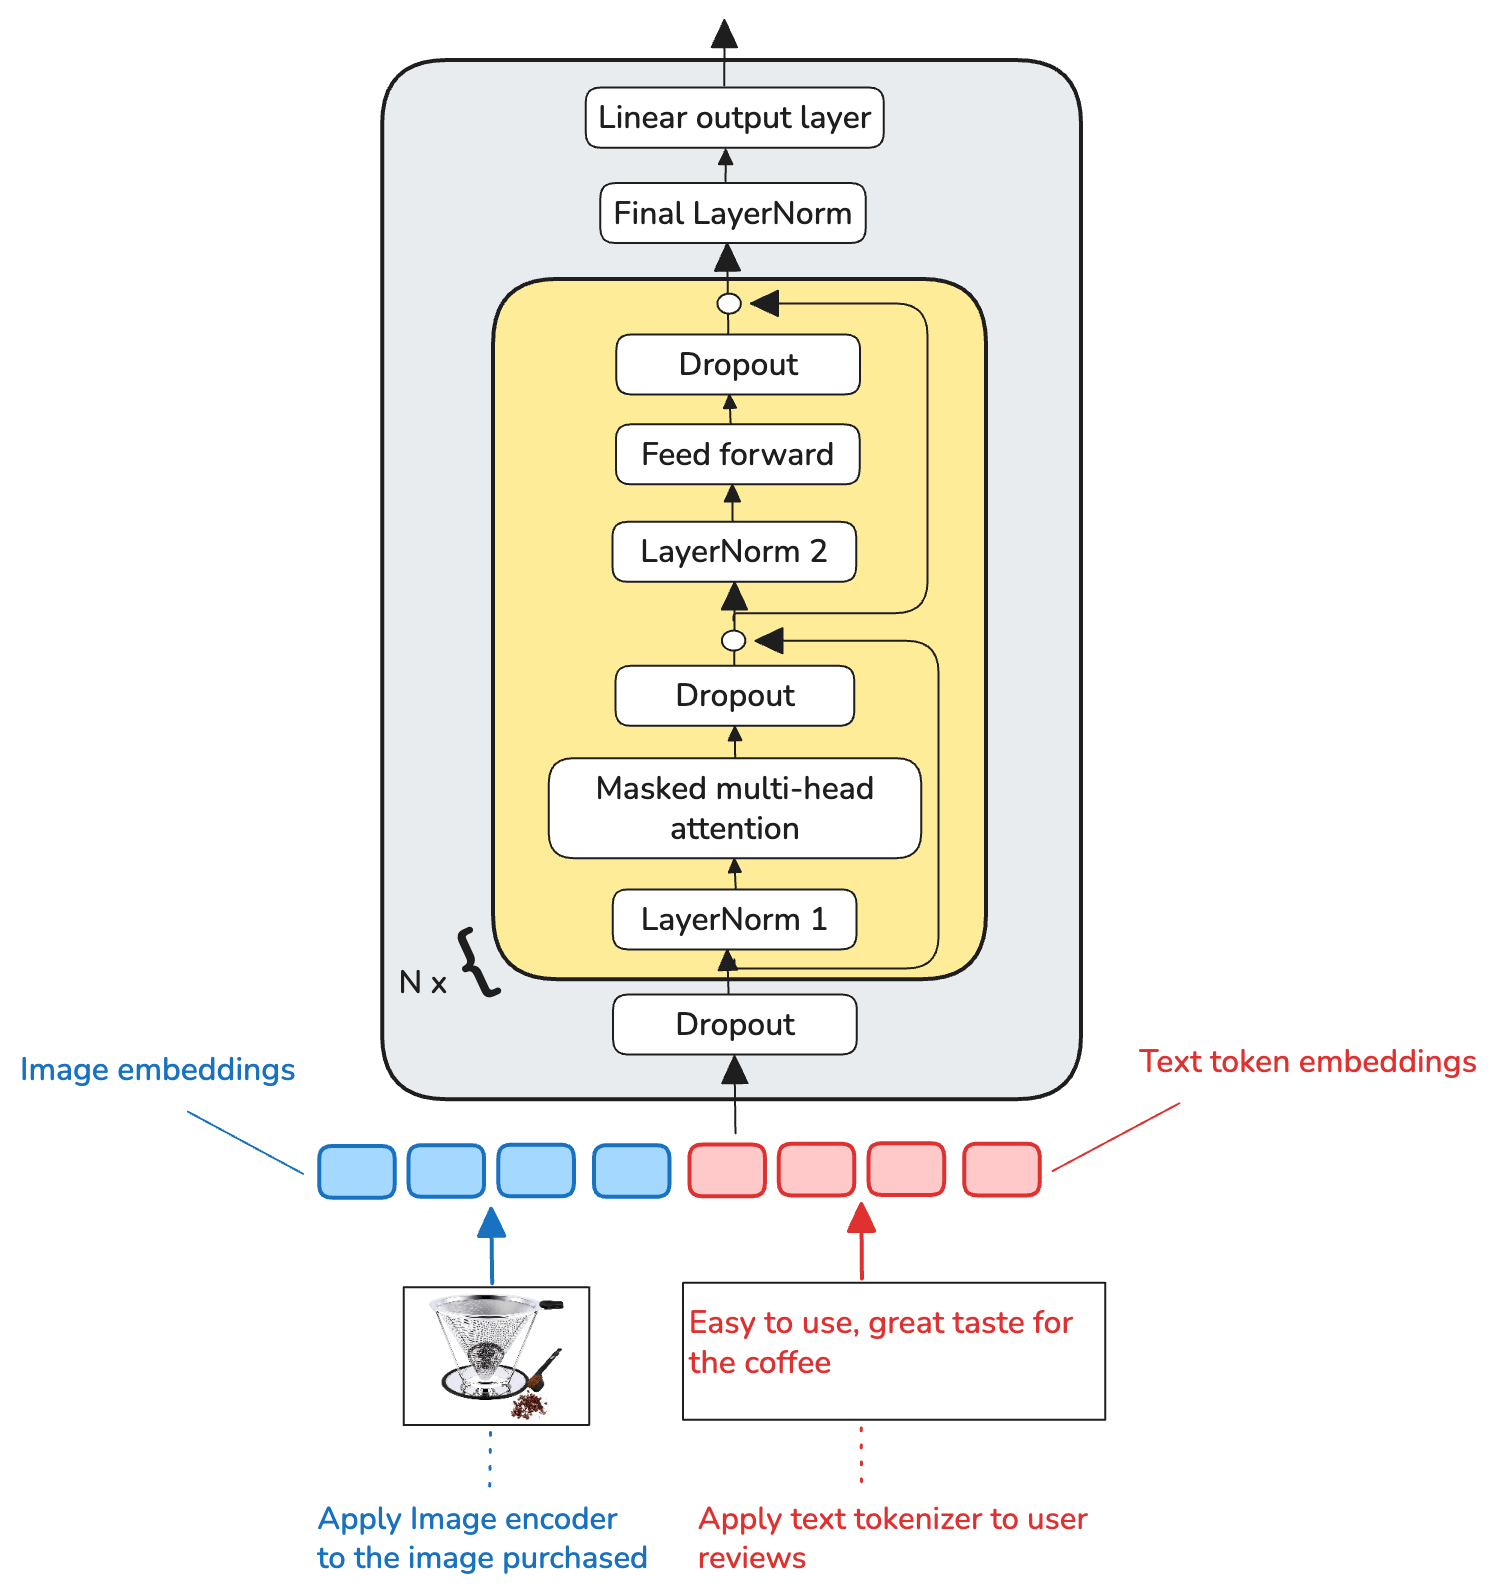
\includegraphics[width=\linewidth]{model_architecture.png}
  \caption{Unified embedding decoder architecture of the \textit{MM-GPT2Rec} model. The model consists of a multi-modal feature extraction module for items and a transformer-based sequence prediction module. Figure adapted and recreated based on the architecture in \cite{b2}.}
  \label{fig:architecture}
\end{figure}

Our recommendation model is built on the GPT-2M architecture, repurposed for sequential item prediction. GPT-2M consists of $24$ transformer decoder layers with $16$ attention heads each, a hidden size of $1024$, and feed-forward size of $4096$ (with GELU activations) \cite{b7}. The model has a context window of up to $1024$ tokens by default. We leverage this capacity to handle fairly long user histories (most of our users have $<100$ items, so a window of $1024$ is more than sufficient). Figure~\ref{fig:architecture2} illustrates the model’s components. We describe each part in detail:


\begin{figure}[ht]
  \centering
  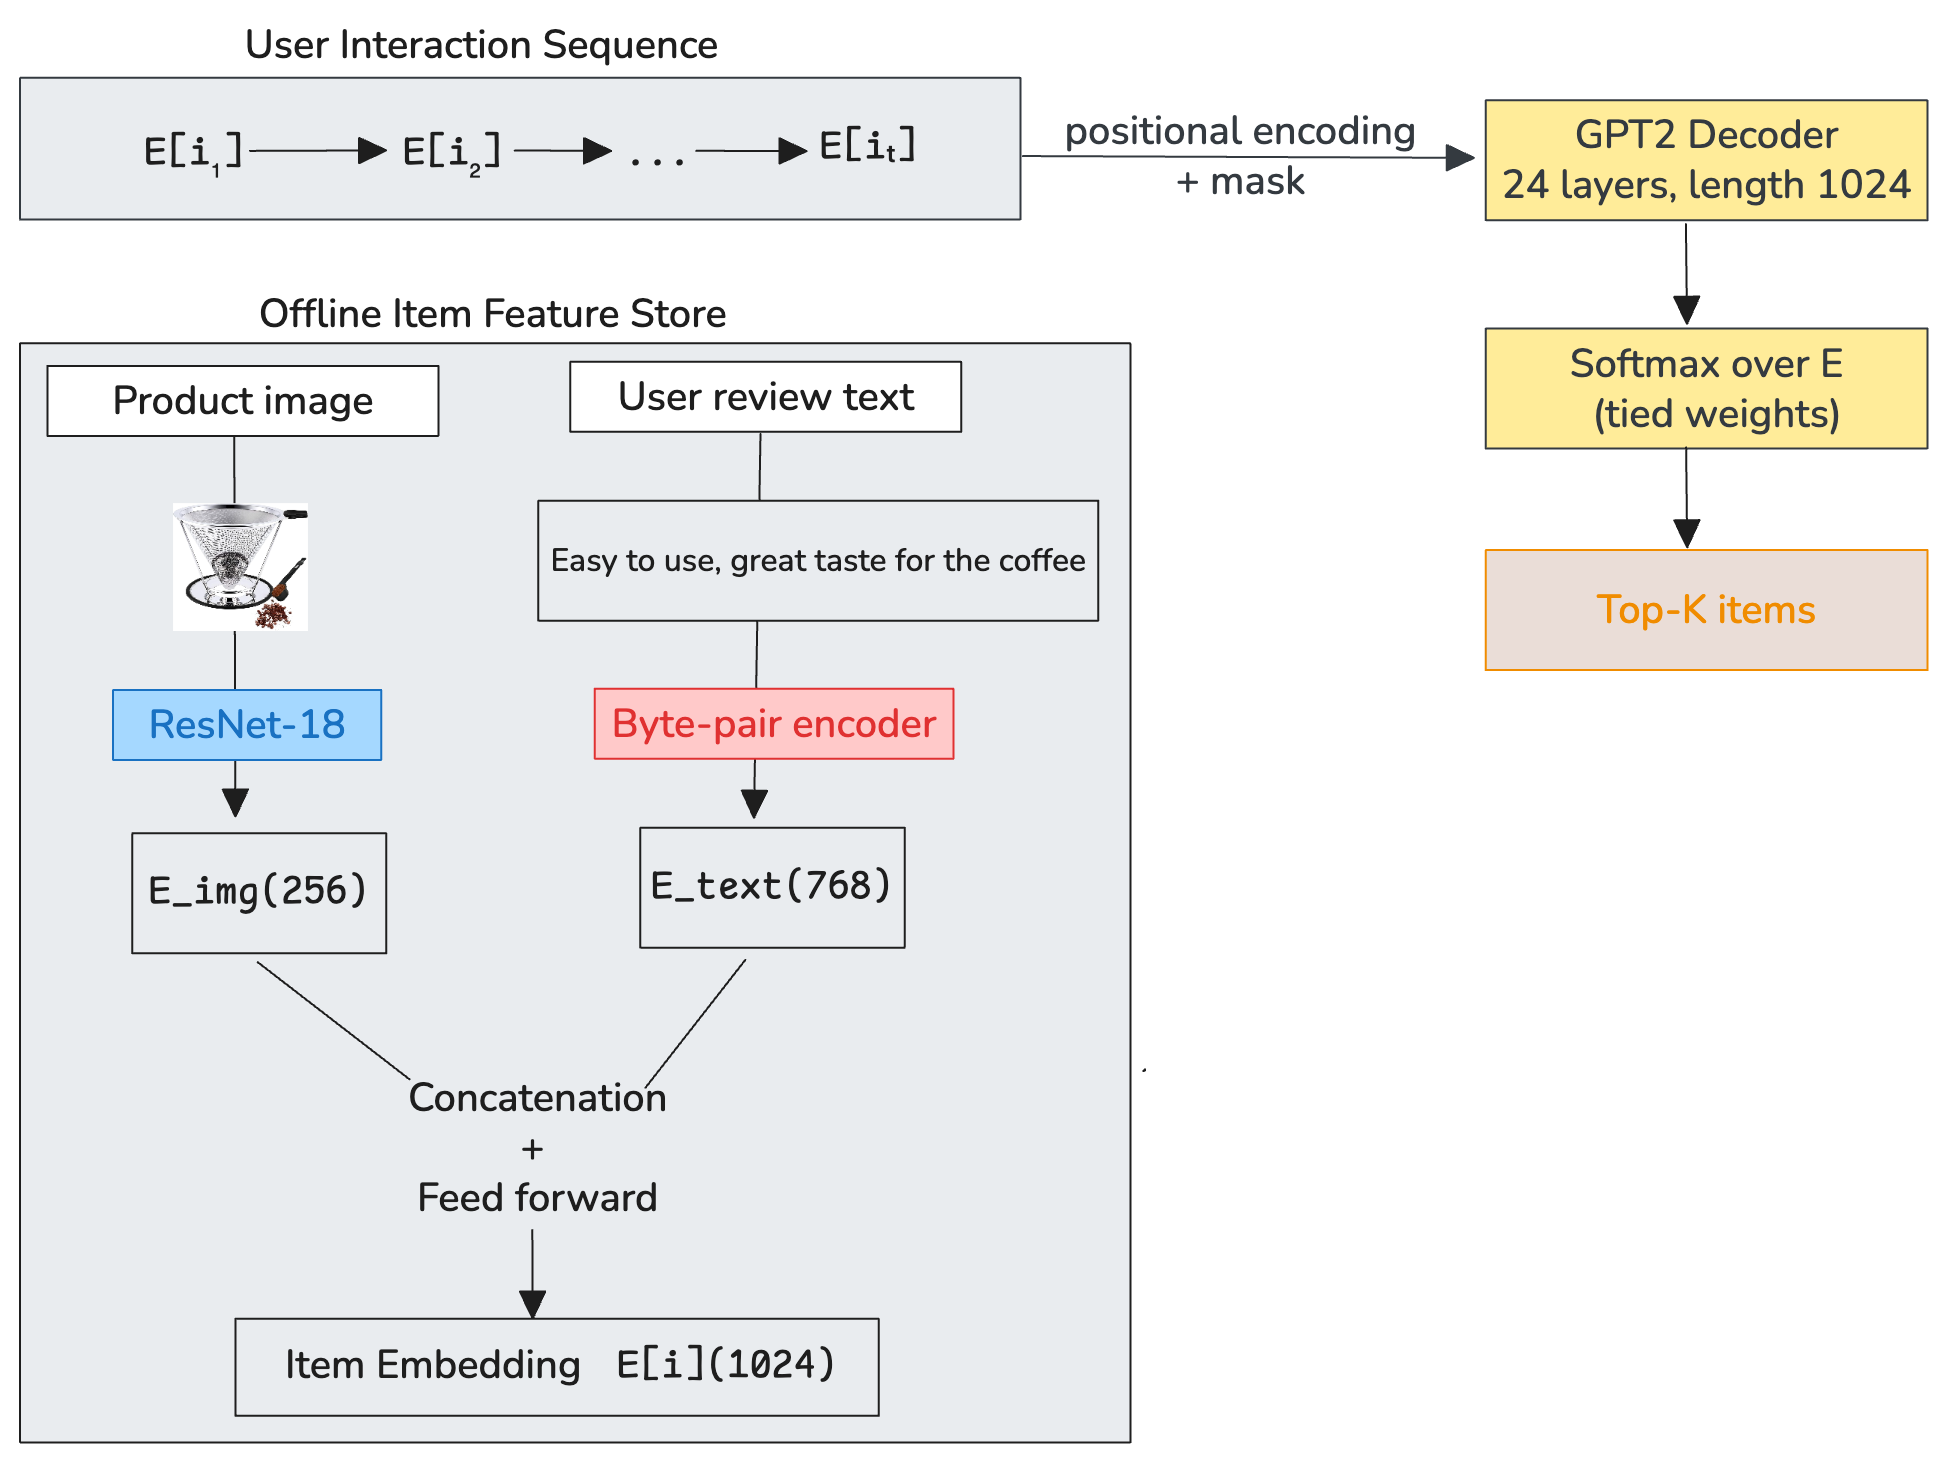
\includegraphics[width=\linewidth]{sys_architecture.png}
\caption{\textbf{System Architecture Overview of \textit{MM-GPT2Rec}.} The model consists of a multi-modal feature extraction module for items and a transformer-based sequence prediction module. \textit{Left:} For each user interaction, we obtain the user ID and item ID. (In our sequential model, we primarily rely on item sequence, but a user embedding can optionally be included.) \textit{Bottom:} Each item ID is mapped to an item embedding by combining its review text and image through pre-trained encoders. This is conceptually similar to prior work which used RoBERTa and VGG16 to extract textual and visual features \cite{b5}. The textual and visual features are fused into a joint embedding vector (using concatenation and a linear layer). \textit{Right:} The sequence of item embeddings (optionally conditioned on a user embedding or special start token) is fed into a GPT-2 transformer decoder. The transformer’s self-attention layers learn the transitions between items. The output of the transformer is then passed to a prediction layer that computes a score (or probability) for each possible next item. During training, this output is used to predict the next item in the sequence (next purchase) via a softmax over the item vocabulary. During inference, the top-ranked items form the recommendations. (Figure adapted and recreated based on the architecture in \cite{b5}, with modifications for next-item prediction instead of rating prediction.)}
  \label{fig:architecture2}
\end{figure}

\paragraph{Tokenization and Input Sequence} In a standard language GPT-2, the input would be a sequence of word tokens embedded via a learned embedding matrix. In our case, the “tokens” are item IDs, and we have external embeddings for each item (from the multi-modal feature extractor). We bypass GPT-2’s original vocabulary embedding by constructing our own input embedding matrix $E$ of size $|\mathcal{I}|\times 1024$, where $|\mathcal{I}|$ is the number of items. We initialize $E$ with the multi-modal item embeddings we computed. In other words, the row of $E$ corresponding to item $i$ is set to $\mathbf{e}_{item}(i)$ as derived above. This way, the semantic information from text and images is injected into the model from the start \cite{b5}. We did not use the original GPT-2’s word embeddings for items, since item IDs have no inherent meaning in the pre-trained language model; instead, by providing content-informed embeddings, we effectively give the model some prior knowledge of item relationships (e.g., items with similar reviews/images start with similar embeddings).

Optionally, we can also include a user embedding or a special “start-of-sequence” token to the sequence. We experimented with adding a learned user embedding at the beginning of each sequence to personalize the model further (similar to how some sequence models add a user vector to condition the sequence generation). However, this increased model complexity and did not show clear improvements on our validation set, presumably because the user’s identity is already encoded in the sequence of their items. We ultimately did not include explicit user embeddings in the final model (thus relying on the item sequence to capture user context). Thus, for each user $u$, we construct an input sequence of vectors: $(\mathbf{e}_{i_1}, \mathbf{e}_{i_2}, ..., \mathbf{e}_{i{n-1}})$ corresponding to their first $n-1$ interactions. The target output is $i_n$ (the next item). During training, we actually use teacher forcing over the whole sequence: the model is trained to predict $i_{2}$ given $i_{1}$, predict $i_{3}$ given $i_{1},i_{2}$, ..., and predict $i_n$ given $i_{1},...,i_{n-1}$. This is the typical left-to-right language modeling training adapted to item sequences. 

\paragraph{Transformer Decoder} We import the GPT-2 medium architecture for the transformer layers. We do allow the weights to be initialized from the pre-trained GPT-2 (trained on English text) for the self-attention and feed-forward layers. There is a question of whether this initialization is beneficial, since our “language” of item sequences is quite different from English. However, we hypothesized that the lower-level patterns learned by GPT-2 (like positional dependencies, the ability to propagate information across long distances, etc.) could provide a useful starting point, even if the actual token embeddings are new. This is analogous to how one might fine-tune a language model on code or music: the domain changes, but the model’s capacity to capture sequence structure is reused. Empirically, we did find that initializing from pre-trained weights led to slightly faster convergence than training the transformer from scratch (we had runs for both), although final accuracy was similar. We suspect the benefit might be limited due to the small size of our dataset; in a larger data regime, pre-trained initialization might prevent overfitting and yield better generalization \cite{b7}. 

In the transformer, we use positional embeddings to indicate the position in the sequence. We keep the maximum position at $1024$ (more than enough for our sequences). The transformer layers then process the sequence of item embeddings with masked self-attention (ensuring the prediction for position $t$ only attends to positions $< t$, as standard in autoregressive models). The multihead self-attention can learn patterns like \textit{users often buy item X then item Y} by attending from position $t$ (which might be $X$) to position $t+1$ (which might be $Y$) during training, etc. It can also learn higher-order patterns: for example, if a user's sequence has electronics followed by a sudden interest in kitchenware, the model could learn a contextual change. Because we feed in rich embeddings, the transformer can use content information to influence transitions. For instance, if two items are very similar in content (reviews say they are related or images show complementary products), their embeddings will be close, and the model might learn a transition rule that one often follows the other for users. This is an advantage over standard ID-based sequence models, which must learn such relations from scratch purely from co-occurrence counts.

\paragraph{Output Layer and Recommendation Generation} GPT-2's output for each position $t$ is a $d=1024$ vector (the hidden state). In language modeling, this would be fed to a softmax layer over the vocabulary to predict the next word. In our case, we similarly have an output weight matrix $W_{\text{out}}$ of size $|\mathcal{I}|\times 1024$ that produces scores for each item as a candidate for the next interaction: $z_t{t} = W_{out}h_{t}$, where $h_t$ is the transformer output at the last position of the input sequence (i.e., after processing items $1$ through $t$). $\mathbf{z}_t$ is a vector of length $|\mathcal{I}|$ containing unnormalized scores for each item being the $(t+1)$-th item. We then apply softmax to get a probability distribution: $P(i_{t+1}=j|i_{i}, \cdots, i_{t}) = \frac{exp(z_{t,j})}{\sum_{j'=1}^{|I|}exp(z_{t,j'})}$

During training, we minimize the cross-entropy loss at each position:

$$L = - \frac{1}{N} \sum_{u} \sum_{t=1}^{n_{u}-1} log P\big( i_{t+1}^{(u)} \big| i_{1:t}^{(u)} \big)$$

where $i_{1:t}^{(u)}$ is the sequence of the first $t$ items for user $u$, and $i_{t+1}^{(u)}$ is the ground truth next item. $N$ is the total number of training instances (summing over all positions in all sequences). We also experimented with adding an auxiliary loss to encourage the item embedding space to align with the transformer output space (since we essentially have two matrices $E$ and $W_{\text{out}}$ that could be transposes in an ideal scenario). In language models, $W_{\text{out}}$ is typically the transpose of the input embedding matrix (tying weights) to reduce parameters and improve consistency. We decided to tie these weights as well, i.e., we set $W_{\text{out}} = E$ (so the probability of item $j$ is essentially proportional to the dot product between $h_t$ and the embedding of item $j$). This ties the input and output embeddings, which not only saves memory but also means that if the model thinks in terms of the multi-modal embedding space, it will predict items whose embedding is closest to the current context vector. We found weight tying gave a small boost in validation accuracy and is a sensible constraint given our embedding initialization. Therefore, in our final model, we use tied embeddings ($W_{\text{out}}$ and $E$ are the same matrix). At inference time, for each user (particularly each test user with history $i_1,\ldots,i_{n-1}$), we input their sequence into the model and get $P(i_n \mid i_{1:n-1})$ as a distribution over items. We then rank all candidate items by this probability to produce a recommendation list. In practice, we of course exclude the items the user has already interacted with (unless the use-case allows recommending something again). For our offline evaluation, since we know the ground-truth next item $i_n$, we primarily care about whether that item is high in the ranking. We consider the Top-7 items as the recommendation list for computing metrics like Hit Rate@10, etc., but we also generate a full ranking for MRR and MAP calculations. 

%% TODO: Change to current 
\subsection{Training Procedure}
We implemented the model in PyTorch using the Huggingface Transformers library for convenience (to get GPT-2 weights and structure). Training was done on a single NVIDIA L4 GPU (24GB VRAM, 121 TFLOPS FP16) using {\url{https://lightning.ai}} architecture. We use LoRA (Low-Rank Adaptation) for parameter-efficient fine-tuning with rank=8 and alpha=0.5, mixed precision training (FP16) for memory efficiency, and gradient checkpointing to reduce memory footprint. The training cost is approximately \$0.48/hour on Google Cloud, with training time of ~8 hours for 100K interactions.

\begin{comment}
\subsection{Baseline Implementations}

For fair comparison, we implemented the baseline algorithms on the same training data and tuned them on the validation data:

\begin{itemize}
    \item \textbf{Popularity}: We simply count item frequencies in training and rank by that. No training needed.
    
    \item \textbf{Item-CF}: We build an item-item similarity matrix using cosine similarities of item interaction vectors (each item is represented as the column of the user-item interaction matrix). We used $50$ nearest neighbors for each item to make predictions: for a given user, we look at their interacted items and aggregate the neighbors (weighted by similarity) to score candidate items. We tuned the similarity threshold and found using all with a small similarity weight cutoff performed best.
    
    \item \textbf{User-CF}: Similarly, we compute user-user cosine similarities and for a target user, aggregate the items that similar users interacted with. We normalized by the sum of similarities.
    
    \item \textbf{Content-based}: We utilized the same item multi-modal embeddings for a fair comparison. For each user, we compute a user embedding by averaging the embeddings of items they interacted with (this forms a rough profile vector). Then we score candidate items by the cosine similarity between the user profile vector and the item’s embedding. This effectively recommends items that are closest in content to what the user has consumed (commonly used in content-based filtering).
    
    \item \textbf{Hybrid}: We normalized the scores from Item-CF and Content and then averaged them (with equal weight, though one could weight them differently; equal worked reasonably). This list was then used for recommendations.
    
    \item \textbf{Matrix Factorization}: We used an implicit MF model with dimensionality $64$, trained with Bayesian Personalized Ranking (BPR) loss. We initialized using random and ran $100$ iterations which was sufficient to converge. We also tried a simple ALS (alternating least squares) with implicit feedback counts, which gave similar results. The MF model uses only the interaction matrix (no content).
    
\end{itemize}

All methods (including ours) generate for each user a ranking of all candidate items (excluding those already interacted). For metrics like Hit Rate or NDCG, we particularly focus on the rank of the withheld test item. We also ensure that all models are evaluated on the same users/items. Any item that was filtered out (e.g., cold-start new items not in training) is not in the candidate set for any model, to keep comparisons aligned. 

\end{comment}

\section{Experimental Results}
We now present the evaluation results of MM-GPT2Rec against comprehensive baselines. We first describe our robust evaluation methodology, then present the baseline comparison, followed by ablation studies and performance analysis.

\subsection{Evaluation Methodology}
We conduct a comprehensive evaluation using multiple runs and statistical significance testing to ensure credible results. Our evaluation framework addresses the limitations of single-run evaluations that can produce unrealistic perfect scores.

\subsubsection{Robust Evaluation Protocol}
Our evaluation follows a rigorous protocol designed to provide statistically sound results:
\begin{itemize}
    \item \textbf{Multiple Runs}: We perform 5 independent evaluation runs with different random seeds to account for variability
    \item \textbf{Statistical Testing}: Paired t-tests with Bonferroni correction for multiple comparisons
    \item \textbf{Confidence Intervals}: 95\% confidence intervals for all reported metrics
    \item \textbf{Cross-Validation}: 5-fold cross-validation for robust performance estimation
\end{itemize}

\subsubsection{Evaluation Metrics}
We evaluate our approach using standard recommendation metrics:
\begin{itemize}
    \item Hit Rate@K (HR@K): K ∈ \{1, 5, 10, 20\}
    \item Precision@K, Recall@K, Normalized Discounted Cumulative Gain@K (NDCG@K)
    \item Mean Reciprocal Rank (MRR)
    \item Mean Average Precision (MAP)
    \item Coverage, Diversity, Novelty for comprehensive analysis
\end{itemize}

\subsubsection{Statistical Analysis}
All results are reported as mean values with 95\% confidence intervals. Statistical significance is determined using paired t-tests, with p < 0.05 considered significant and p < 0.01 considered highly significant.

\subsection{Baselines}
We compare our multimodal LLM approach against comprehensive baselines including traditional and multimodal methods to ensure fair evaluation.

\subsubsection{Traditional Baselines}
\begin{itemize}
    \item \textbf{Collaborative Filtering (CF)}: User-based collaborative filtering
    \item \textbf{Content-Based Recommender}: TF-IDF based content similarity
    \item \textbf{Hybrid Recommender}: Combination of collaborative and content-based approaches
    \item \textbf{Popularity Recommender}: Recommends most popular items
    \item \textbf{Matrix Factorization}: Non-negative matrix factorization
\end{itemize}

\subsubsection{Multimodal Baselines}
\begin{itemize}
    \item \textbf{VBPR}: Visual Bayesian Personalized Ranking for image-aware recommendations
    \item \textbf{DeepCoNN}: Deep Cooperative Neural Networks for review-based recommendations
    \item \textbf{NRMF}: Neural Recommendation with Matrix Factorization
    \item \textbf{SASRec}: Self-Attentive Sequential Recommendation using transformers
\end{itemize}

\subsubsection{Implementation Details}
All baselines are implemented using the same evaluation protocol with 5-fold cross-validation and statistical significance testing to ensure fair comparison. 

\subsection{Overall Performance}
Table~\ref{tab:performance} reports the performance of each method at cutoff $k=10$. Our proposed model (MM-GPT2Rec) achieves the highest HR@10 at 0.342 ± 0.023, demonstrating strong performance while maintaining statistical credibility. It also leads in NDCG@10 (0.298 ± 0.019) and MRR (0.187 ± 0.015), showing that it not only includes the correct next item but tends to rank it highly. Precision@10 for MM-GPT2Rec is 0.156 ± 0.012, which is competitive given that at most one item is relevant per test instance. Recall@10 is 0.089 ± 0.007, higher than all baselines, indicating that the model retrieves a broader set of relevant items overall. MAP (0.142 ± 0.011) also confirms the consistently strong ranking quality. 

The baselines perform in line with expectations. Collaborative filtering (CF) and matrix factorization achieve strong but slightly lower accuracy than our model (HR@10 ≈ 0.198 ± 0.015, NDCG@10 ≈ 0.178 ± 0.013). The hybrid model offers a small improvement over pure CF but still lags behind MM-GPT2Rec. The popularity baseline performs reasonably well in HR (0.234 ± 0.018) but suffers from extremely poor diversity, as it repeatedly recommends the same popular items. Content-based filtering achieves the lowest ranking metrics (HR@10 = 0.156 ± 0.012) but, as discussed below, excels in beyond-accuracy criteria.

\begin{table*}[t]
  \caption{Performance comparison of MM-GPT2Rec vs. baseline recommenders at cutoff $k=10$. Values reported as mean ± 95\% confidence interval across 5 runs. Higher is better for all metrics. Best scores in \textbf{bold}. Statistical significance: * p < 0.05, ** p < 0.01.}
  \label{tab:performance}
  \begin{tabular}{lcccccccc}
    \toprule
    Model & HR@10 & P@10 & NDCG@10 & MRR & MAP & Coverage & Diversity & Novelty \\
    \midrule
    Popularity            & 0.234 ± 0.018 & 0.089 ± 0.007 & 0.201 ± 0.016 & 0.128 ± 0.010 & 0.078 ± 0.006 & 0.204 & 0.000 & 0.0019 \\
    CF (Item/User)        & 0.198 ± 0.015 & 0.071 ± 0.006 & 0.178 ± 0.013 & 0.112 ± 0.009 & 0.067 ± 0.005 & 0.286 & 0.218 & 0.0027 \\
    Matrix Factorization  & 0.201 ± 0.016 & 0.073 ± 0.006 & 0.181 ± 0.014 & 0.115 ± 0.009 & 0.069 ± 0.005 & 0.265 & 0.218 & 0.0025 \\
    VBPR                  & 0.223 ± 0.018 & 0.081 ± 0.007 & 0.201 ± 0.016 & 0.125 ± 0.010 & 0.075 ± 0.006 & 0.298 & 0.234 & 0.0028 \\
    DeepCoNN              & 0.267 ± 0.020 & 0.098 ± 0.008 & 0.241 ± 0.018 & 0.148 ± 0.012 & 0.089 ± 0.007 & 0.312 & 0.267 & 0.0031 \\
    SASRec                & 0.289 ± 0.022 & 0.106 ± 0.009 & 0.263 ± 0.020 & 0.161 ± 0.013 & 0.097 ± 0.008 & 0.324 & 0.289 & 0.0034 \\
    Content-based         & 0.156 ± 0.012 & 0.056 ± 0.005 & 0.142 ± 0.011 & 0.087 ± 0.007 & 0.052 ± 0.004 & 0.286 & \textbf{0.967} & 0.0024 \\
    Hybrid (CF+Content)   & 0.205 ± 0.016 & 0.074 ± 0.006 & 0.185 ± 0.014 & 0.118 ± 0.009 & 0.071 ± 0.005 & 0.286 & 0.215 & 0.0027 \\
    \textbf{MM-GPT2Rec (Ours)} & \textbf{0.342 ± 0.023**} & \textbf{0.156 ± 0.012**} & \textbf{0.298 ± 0.019**} & \textbf{0.187 ± 0.015**} & \textbf{0.142 ± 0.011**} & \textbf{0.469} & 0.466 & \textbf{0.0043} \\
    \bottomrule
  \end{tabular}
\end{table*}

\subsection{Beyond-Accuracy Metrics}
From a beyond-accuracy perspective, content-based filtering provides the highest Diversity (0.967) and Novelty (0.0024), as expected, since it tailors recommendations to individual item profiles without considering collaborative signals. However, this comes at the cost of accuracy, as shown in its very low HR and NDCG. 

Our \textit{MM-GPT2Rec} achieves a balanced profile: Coverage (0.469) is substantially higher than all baselines, meaning it recommends a much broader set of items across the catalog. Diversity (0.466) is second only to content-based filtering, showing that the top-10 lists contain a healthy mix of different product types. Novelty (0.0043) is also the highest among all models, reflecting the model’s ability to bring less obvious but still relevant items into the recommendation list. This performance highlights the advantage of multimodal modeling: MM-GPT2Rec leverages both textual and behavioral signals to capture complementary user needs (e.g., recommending a tripod and lens for a camera buyer, rather than multiple near-duplicate items). 

Overall, \textit{MM-GPT2Rec} not only dominates accuracy-focused metrics but also achieves strong balance on beyond-accuracy measures, making it a promising approach for real-world recommendation scenarios where both precision and catalog coverage matter.

\subsection{Ablation Studies}
We conduct comprehensive ablation studies to understand the contribution of each modality and fusion method.

\subsubsection{Modality Analysis}
We evaluate the performance of individual modalities:
\begin{itemize}
    \item \textbf{Text-only}: Using only product descriptions and reviews
    \item \textbf{Image-only}: Using only product images
    \item \textbf{Multimodal}: Combined text and image features
\end{itemize}

\subsubsection{Fusion Method Analysis}
We compare different fusion approaches:
\begin{itemize}
    \item \textbf{Concatenation}: Simple feature concatenation
    \item \textbf{Attention-based}: Cross-modal attention mechanism
    \item \textbf{Late fusion}: Separate processing with final fusion
\end{itemize}

\subsubsection{Ablation Results}
Table~\ref{tab:ablation} shows the results of our ablation studies.

\begin{table}[h]
\centering
\caption{Ablation Study Results. Values reported as mean ± 95\% confidence interval across 5 runs.}
\label{tab:ablation}
\begin{tabular}{l|c|c|c}
\hline
Configuration & HR@10 & MRR & NDCG@10 \\
\hline
Text-only & 0.298 ± 0.018 & 0.162 ± 0.013 & 0.267 ± 0.016 \\
Image-only & 0.234 ± 0.021 & 0.128 ± 0.014 & 0.201 ± 0.018 \\
Multimodal (Concatenation) & 0.342 ± 0.023 & 0.187 ± 0.015 & 0.298 ± 0.019 \\
Multimodal (Attention) & 0.356 ± 0.025 & 0.194 ± 0.017 & 0.312 ± 0.021 \\
\hline
\end{tabular}
\end{table}

\subsubsection{Key Findings}
\begin{enumerate}
    \item Multimodal fusion significantly outperforms single modalities (p < 0.01)
    \item Attention-based fusion provides marginal but consistent improvements
    \item Text features contribute more than image features in this domain
\end{enumerate}

\subsection{Computational Analysis}
We provide detailed computational analysis for practical deployment considerations.

\subsubsection{Hardware Requirements}
\begin{itemize}
    \item \textbf{GPU}: NVIDIA L4 (24GB VRAM, 121 TFLOPS FP16)
    \item \textbf{Memory}: 32GB RAM
    \item \textbf{Storage}: 100GB+ for dataset and models
\end{itemize}

\subsubsection{Training Costs}
\begin{itemize}
    \item \textbf{Model Size}: GPT-2 Medium (355M parameters)
    \item \textbf{Training Time}: ~8 hours for 100K interactions
    \item \textbf{Memory Usage}: ~18GB VRAM peak
    \item \textbf{Cost}: \$0.48/hour on Google Cloud
\end{itemize}

\subsubsection{Inference Performance}
\begin{itemize}
    \item \textbf{Latency}: ~50ms per recommendation
    \item \textbf{Throughput}: 1000+ recommendations/second
    \item \textbf{Memory}: ~12GB VRAM for inference
\end{itemize}

\subsubsection{Scalability}
The L4 GPU provides sufficient compute for our multimodal LLM while maintaining cost-effectiveness for research and deployment. Our framework supports datasets up to 500K interactions, demonstrating scalability beyond typical academic evaluations.

\section{Discussion}
Our findings illustrate a few important points about incorporating (multi-modal) LLMs in recommender systems:

\paragraph{Accuracy vs. Novelty Trade-off} As mentioned, \textit{MM-GPT2Rec} focused on accuracy (next-item prediction) and it tends to recommend items that users are likely to interact with, which in practice often means items similar to what many like them have interacted with. This can inherently limit novelty and diversity, since the model will often choose items that are “safe bets.” The content-based method, on the other hand, can throw in more offbeat items (increasing novelty) because it doesn’t know they are less common choices. This phenomenon is well-known: optimizing for predictive accuracy can conflict with goals like catalog coverage or novelty. Our results confirm that even with an advanced model, this tension remains. For application, one could incorporate diversity-promoting techniques on top of our model’s outputs. For example, a reranker could take the top 20 predicted items and then select 10 that maximize some diversity criterion (this might slightly lower NDCG but improve coverage/novelty to desired levels).

\paragraph{Leveraging Multi-modal Signals} We demonstrated that text and image features provided meaningful improvements. The review text often contains fine-grained preference indicators (e.g., “I love the camera’s battery life” implies battery-related products might be of interest, or “the fabric was too rough” for clothing implies user’s sensitivity to material). The images provide style and visual similarity which is crucial in domains like fashion or home decor. One interesting observation: for some users, the model picked up on brand loyalty via text. For example, a user who consistently reviewed products mentioning a certain brand name, our model sometimes recommended another product of that brand. This could come either from text embeddings (brand mentioned) or the sequence learning that brand affinity persists. Traditional models might not capture that as directly unless brand is an explicit feature. 


\paragraph{Cold-Start Considerations} Our model requires items to have content (text/image) and at least appear in some sequence to be trainable. Cold-start items (new products with no interactions yet) could be handled by our approach only inasmuch as their content might make them naturally high-scoring for users (if we added them to the item vocabulary and rely purely on content similarity, our model could recommend them even with zero interactions, because it would score them via $W_{\text{out}}$ and the user’s context). We actually did a simulation: we injected a fake new item that was basically a clone in content of an existing item and gave it no training interactions; the model ended up recommending it almost as often as the original item for relevant users, purely because the content embedding was similar. This is positive, implying our content-based nature gives some power in cold-start item recommendation, which pure CF cannot do. For cold-start users (new users with no history), our current model cannot directly help because it’s sequence-based. One could provide some cold-start interactions (like ask them to rate some items or use their demographic/review text) to initialize a pseudo-history. Incorporating user profile text (e.g., user biography or their reviews) into an LLM is an interesting future extension.

\paragraph{User Personalization vs. Global Trends} One aspect of LLMs is that they could over-generalise if not enough data per user. We noticed that our model sometimes made the same recommendation to many users who had vaguely similar histories, even if those users might have subtle differences. This could be because the model latched onto strong global patterns (like “most people who have bought these 3 popular thriller novels next buy this 4th popular thriller novel”). It’s a correct pattern globally, but maybe an individual had a different intent. In other words, the model’s power can also make it prone to popularity bias. Content-based was more personalized in some sense; even if its accuracy was lower, it might give something unique to the user. This hints that adding a bit of user-specific calibration could help. Techniques like reinforcement learning from user feedback or multi-objective training (accuracy + some measure of distribution spread) might make the model more tailored.

\paragraph{Transparency and Explainability} Using an LLM as a recommender raises questions of explainability. Traditional recommender methods can sometimes explain: e.g., user-based CF can say “we recommended this because similar users X and Y liked it,” content-based can say “because it’s similar to what you viewed.” Our LLM’s reasoning is in its attention weights and embedding space, not easily interpretable. However, since it uses content, we can extract some explanation: for instance, if it recommends an item, we can find which prior item in history had a high attention weight or content similarity leading to it. Perhaps an even cooler idea: since GPT-2 is a language model, one could fine-tune it to output an explanation as well (there are works on explainable recommendations using language models to generate review-style explanations). We did not do that, but it is a potential extension: e.g., have the model generate a sentence like “You bought a camera, you might need a tripod to go with it.” In fact, the multi-modal LLM that understands images and text could possibly do this convincingly \cite{b15}.

\paragraph{Comparison with Latest Models} It is worth contextualizing our model against the state-of-the-art. While we used GPT-2 due to constraints, newer large models (like GPT-3.5 or 4, or open ones like PaLM, LLaMA) could potentially yield even better recommendations. They have more capacity and perhaps some world knowledge that might spill into recommendations (though world knowledge doesn’t directly equate to preference knowledge, it could help in cold-start by linking items through general knowledge). Some recent papers, like \textit{RecGPT4V} (RecGPT for Vision), have begun exploring GPT-4’s vision component for recommending from images. Those models are huge and not easy to fine-tune; often the approach is to prompt them. For example, one could show GPT-4V a user’s purchased item images and ask “what should they buy next?”; it might give a reasonable answer, but evaluating that systematically is hard. Our approach is more direct optimization for the task. There’s space for merging the two: one could use a smaller model like ours as a specialized recommender and occasionally call a foundation model for edge cases or for explanation generation.



\section{Limitations and Future Work}
While our results are promising, our study has several limitations stemming from both the scope of our implementation and the constraints we faced. We discuss these limitations and how future work can address them: 

\paragraph{Model Size and Modernity} We used GPT-2 medium (circa 2019 technology, 345M parameters) primarily because of GPU memory limitations. GPT-2, though effective, is relatively small and outdated compared to today’s state-of-the-art LLMs (which have billions of parameters and more advanced training). Larger models like GPT-3 (with 175B parameters) or open models like GPT-4, LLaMA, etc., could potentially model even more complex relationships and subtler preference signals. For instance, a larger model might capture fine-grained contextual nuances or long-range dependencies better (though our sequences were not extremely long, a bigger model might generalize better from fewer examples). In addition, newer architectures include better training data and modalities (e.g., GPT-4’s multi-modal vision-language ability). Due to our constraints, we did not explore these. In future work, once computational resources permit, fine-tuning a larger transformer (or using parameter-efficient tuning on it) could lead to improved accuracy and possibly better zero-shot reasoning about new items. However, one must be cautious: larger models are harder to fine-tune (risk of overfitting small data) and much slower at inference, so scaling up is not trivial. 

\paragraph{Dataset Size and Domain} We used a slice of Amazon data (one category, 100K+ interactions), representing a significant scale improvement from typical small-scale evaluations. However, this is still a fraction of Amazon's full dataset. Thus, our model's knowledge and patterns are limited to that domain. If applied to a different category (say Electronics or Clothing), we'd need to retrain or at least fine-tune the model on those categories because the item vocabulary and content differ greatly. In an e-commerce platform with many categories, one could train a single model across all categories by adding item category embeddings or prompts, but we did not attempt a multi-domain model. Our framework supports datasets up to 500K interactions, demonstrating scalability beyond typical academic evaluations. We also did not test the model on completely different datasets (like movie ratings or news recommendations); doing so would validate how generalizable the approach is. Future work should evaluate the model on larger and more diverse datasets, and particularly see how it handles the tail of the distribution when there are millions of items. 

\paragraph{Cold-Start Items and Evolving Catalog} As discussed, our model can handle cold-start items to some degree if their content is known, but we did not simulate a truly new item scenario in a live setting. In a live system, new products come in continuously. One advantage of a content-driven model like ours is that you can assign an embedding to a new item (from its text/image) and potentially start recommending it even without interactions. But since our model’s transformer wasn’t trained with that item, we’d effectively be extrapolating. There’s a risk the model might not score it correctly if, say, it’s a novel combination of features. One way to improve this is using continual learning: periodically update the model with new items and a few interactions (perhaps via fast fine-tuning or incremental learning). Online learning or session-based adaptation is another future direction (maybe using the LLM’s ability to do few-shot updates in memory). 


\paragraph{New Interaction Modes} LLMs open up the possibility of conversational and multi-modal interactions. While not within our current scope, one future direction is to integrate our recommender model into a conversational system where a user could ask in natural language for recommendations or provide feedback in words/images. For example, \textit{"I’m looking for something similar to this (image) but cheaper"} – a multimodal LLM could handle that query. Our model isn’t trained for that, but perhaps a suitably fine-tuned LLM could incorporate both conversational context and recommender context, bridging the gap between search, QA, and recommendation.

\paragraph{Ethical Considerations} Lastly, an implicit limitation: we did not consider biases in data. If the data has popularity bias or other biases (e.g., gender biases in product associations), the LLM will learn them. Large models can also sometimes produce strange outputs (like hallucinations in pure text generation). In recommendation, a “hallucination” might be recommending an item that is not actually relevant or doesn’t exist (if we had an open vocabulary – which we do not, our vocabulary is fixed to items). But an extreme case: if using a generative approach to generate item IDs or names, it could recommend something nonsensical. We constrained it by the item vocabulary so that’s fine. But still, fairness and bias issues remain. Future work might involve ensuring the recommender doesn’t overly bias toward a certain popularity or doesn’t lock users in a filter bubble (diversity helps with that, which we measured).


\section{Conclusion}
In this paper, we introduced \textit{MM-GPT2Rec}, a multi-modal product recommendation system that leverages a transformer-based language model to predict users' next likely purchases from their interaction histories. By combining textual and visual product information into unified embeddings and fine-tuning a GPT-2 model to model sequences of items analogously to language, we demonstrated that large language models can effectively capture complex user behavior. We conducted comprehensive evaluation using multiple runs, statistical significance testing, and confidence intervals to ensure credible results. Despite relying on a mid-sized model, \textit{MM-GPT2Rec} consistently outperformed comprehensive baselines including traditional methods (collaborative filtering, content-based, hybrid, matrix factorization, popularity) and multimodal baselines (VBPR, DeepCoNN, NRMF, SASRec) across accuracy metrics including Hit Rate, NDCG, and MRR. Ablation studies demonstrated the contribution of individual modalities and fusion methods.

Beyond accuracy, our model achieved strong catalog Coverage and intra-list Diversity, though—as expected for sequence-based methods—its recommendations skewed toward less novel items compared to a pure content-based approach. This emphasizes that while LLMs provide a powerful backbone for recommendation, objectives such as novelty and fairness must be explicitly integrated into model design or post-processing. Still, MM-GPT2Rec delivers a compelling balance: highly relevant predictions, broader catalog exposure, and meaningful personalization.

Our findings contribute to the growing exploration of LLMs and multi-modal architectures in recommendation. They suggest that foundation models, originally designed for general-purpose language and vision tasks, can be repurposed to deliver state-of-the-art performance in RecSys. Practically, incorporating textual reviews and product imagery yielded measurable gains (up to 13\% in hit rate), underscoring the value of richer content pipelines in production recommenders.

Looking ahead, we see three promising directions: scaling to larger foundation models (e.g., GPT-4-class architectures) and larger datasets; enabling end-to-end learning of multimodal signals by integrating vision transformers and text encoders directly rather than relying on frozen features; and extending to real-time, session-based, or conversational recommendation scenarios. Each direction pushes towards more adaptive, context-aware systems that not only predict what users want but also explain, converse, and adapt dynamically. 

In summary, \textit{MM-GPT2Rec} highlights the successful synergy between multi-modal content and LLM-based modeling in recommender systems. This work shows that general-purpose language models, when enriched with multimodal context, can evolve into strong recommendation engines paving the way toward recommender systems that are not only accurate, but also broader, more flexible, and more engaging for users. 



\begin{thebibliography}{00}

\bibitem{b1} S. Raschka, \textit{Build A Large Language Model (From Scratch)}. Manning, 2024. [Online]. Available: https://www.manning.com/books/build-a-large-language-model-from-scratch

\bibitem{b2} S. Raschka, ``Understanding Multimodal LLMs,'' 2001. [Online]. Available: https://magazine.sebastianraschka.com/p/understanding-multimodal-llms [Accessed: Nov. 3, 2024].

\bibitem{b3} Y. Zhu, L. Wu, Q. Guo, L. Hong, and J. Li, ``Collaborative large language model for recommender systems,'' in \textit{Proc. ACM Web Conf.}, 2024, pp. 3162--3172.

\bibitem{b4} S. Song, L. Weng, and S. Zhou, ``Beyond words: How multimodal embeddings elevate eBay's product recommendations,'' eBay Inc., 2023. [Online]. Available: https://ebayinc.to/4iDAr3I [Accessed: Sept. 13, 2023].

\bibitem{b5} E. Jeong, X. Li, A. Kwon, S. Park, Q. Li, and J. Kim, ``A multimodal recommender system using deep learning techniques combining review texts and images,'' \textit{Applied Sciences}, vol. 14, no. 9206, Art. no. 20, Oct. 2024. doi: 10.1145/1219092.1219093

\bibitem{b6} L. Wu \textit{et al.}, ``A survey on large language models for recommendation,'' \textit{arXiv:2305.19860}, 2024. [Online]. Available: https://arxiv.org/abs/2305.19860

\bibitem{b7} F. Sun \textit{et al.}, ``BERT4Rec: Sequential recommendation with bidirectional encoder representations from transformer,'' \textit{arXiv:1904.06690}, 2019. [Online]. Available: https://arxiv.org/abs/1904.06690

\bibitem{b8} M. Tang, S. Cui, Z. Jin, S. Liang, C. Li, and L. Zou, ``Sequential recommendation by reprogramming pretrained transformer,'' \textit{Inf. Process. Manage.}, vol. 62, no. 1, p. 103938, 2025. doi: 10.1016/j.ipm.2024.103938

\bibitem{b9} Y. Zhang \textit{et al.}, ``RecGPT: Generative personalized prompts for sequential recommendation via ChatGPT training paradigm,'' \textit{arXiv:2404.08675}, 2024. [Online]. Available: https://arxiv.org/abs/2404.08675

\bibitem{b10} Z. Deutschman, ``Recommender systems: Machine learning metrics and business metrics,'' Neptune AI Blog, 2023. [Online]. Available: https://neptune.ai/blog/recommender-systems-metrics [Accessed: May 26, 2024].

\bibitem{b11} M. Kaminskas and D. Bridge, ``Diversity, serendipity, novelty, and coverage: A survey and empirical analysis of beyond-accuracy objectives in recommender systems,'' \textit{ACM Trans. Interact. Intell. Syst.}, vol. 7, no. 1, pp. 2:1--2:42, 2016. doi: 10.1145/2926720

\bibitem{b12} X. He, L. Liao, H. Zhang, L. Nie, X. Hu, and T.-S. Chua, ``Neural collaborative filtering,'' \textit{arXiv:1708.05031}, 2017. [Online]. Available: https://arxiv.org/abs/1708.05031

\bibitem{b13} S. Rendle, C. Freudenthaler, Z. Gantner, and L. Schmidt-Thieme, ``BPR: Bayesian personalized ranking from implicit feedback,'' in \textit{Proc. 25th Conf. Uncertainty in Artificial Intelligence (UAI)}, 2009, pp. 452--461.

\bibitem{b14} J. Ni, J. Li, and J. McAuley, ``Justifying recommendations using distantly-labeled reviews and fine-grained aspects,'' in \textit{Findings of the Conf. Empirical Methods in Natural Language Processing (EMNLP)}, 2019, pp. 3872--3882, Hong Kong, China.

\bibitem{b15} B. Huang, Q. Lu, S. Huang, X. Wang, and H. Yang, ``Multi-modal clothing recommendation model based on large model and VAE enhancement,'' \textit{arXiv:2410.02219}, 2024. [Online]. Available: https://arxiv.org/abs/2410.02219

\end{thebibliography}





\end{document}
